\documentclass[landscape, 25pt]{tikzposter}
\usetikzlibrary{arrows.meta}


%------------------------------------------
% Fonts
%------------------------------------------
\usepackage[T1]{fontenc}
%\usepackage{lmodern} removed lmodern b/c itmesses up sums
\usepackage{textcomp}
%\renewcommand*{\sfdefault}{lmss} % other sf fonts: cmss, lmss, pag, phv
\renewcommand{\familydefault}{\sfdefault}
\usepackage{xcolor}
\usepackage{array}
\usepackage{graphicx}
%------------------------------------------
% Poster options & visual elements
%------------------------------------------
\geometry{paperwidth=36in,paperheight=48in}
\usetheme{Autumn}
\usecolorstyle{Denmark}
\useblockstyle{Default}
\useinnerblockstyle{Default}
\setlength{\textwidth}{48in}
\let\oldblock\block
\renewcommand{\block}[2]{\oldblock{\huge #1}{\Large #2}}

% colors

\definecolor{darkred}{HTML}{7A0000}

\colorlet{titlebgcolor}{darkred}

\colorlet{blocktitlefgcolor}{darkred}
\colorlet{innerblocktitlebgcolor}{darkred}



% theorem boxes, etc.
\newcommand{\theorem}[1]{\innerblock{Theorem}{#1}}
\newcommand{\namedtheorem}[2]{\innerblock{Theorem (#1)}{#2}}
\newcommand{\cor}[1]{\innerblock{Corollary}{#1}}
\newcommand{\defbox}[1]{\innerblock{Definition}{#1}}
\newcommand{\prop}[1]{\innerblock{Proposition}{#1}}
\newcommand{\conj}[1]{\innerblock{Conjecture}{#1}}
\newcommand{\lem}[1]{\innerblock{Lemma}{#1}}


%------------------------------------------
% Bibliography
%------------------------------------------
\usepackage[backend=bibtex]{biblatex}
\addbibresource{pairwise.bib}

%------------------------------------------
% Math-related packages and commands
%------------------------------------------
\usepackage{amsmath,amssymb,amsthm}
\DeclareMathOperator{\disc}{disc}
\newcommand{\setof}[2]{\left\{ #1 \, : \, #2 \right\}}
\newcommand{\Z}{\mathbb{Z}}
\renewcommand{\subset}{\subseteq}
\renewcommand{\supset}{\supseteq}
\newcommand{\B}{\mathcal{B}}
\newcommand{\R}{\mathbb{R}}
\newcommand{\boldp}{\boldsymbol{p}}
\usepackage{xfrac}

%------------------------------------------
% Title information
%------------------------------------------
\title{Generalizations of Conway's Thrackle Conjecture}

\vspace{10in}
\author{
    \begin{tabular}{cccccc}
	\parbox{7in}{\centering Ryan Chen\\ 	\Large Princeton University} &   
	\parbox{7in}{\centering Florian Frick\\ 	\Large Cornell University} & 
	\parbox{7in}{\centering Frederick Huang\\ 	\Large Cornell University} &
	\parbox{7in}{\centering Maxwell Polevy\\ 	\Large Northeastern University} & 
	\parbox{7in}{\centering David Stoner\\ 		\Large Harvard University} & 
	\parbox{7in}{\centering Zoe Wellner \\ 	\Large Cornell University}
\end{tabular}
}


%------------------------------------------
% Begin Document
%------------------------------------------
\begin{document}
\maketitle[titlegraphictotitledistance=-1cm] % rescale title in class file b/c option for it doesn't work
\begin{columns}
%------------------------------------------
% First column
%------------------------------------------
    \column{0.3}
    
    \block{Background}{
    
    \defbox{
             A \emph{thrackle} is a graph drawn in the plane such that any pair of distinct edges intersect precisely once, either at a common vertex or a transverse intersection point.
        }
        \vspace{0.2in}
	    Conway conjectured that for any thrackle the number of edges does not exceed the number of vertices.
	    This is simple to prove if all
    edges are straight line segments, see Erd\H os~\cite{erdos1946},     but is open in general. Lov\'asz, Pach, and Szegedy~\cite{lovasz1997} 
    proved that any 
    thrackle on $n$ vertices has at most $2n-3$ edges. This bound was improved to roughly $1.428n$ by 
    Fulek and Pach~\cite{fulek2010}.
    
    \vspace{0.2in}
    
        We prove convex-geometric analogs of Conway's conjecture and establish bounds on the number of facets for higher-dimensional generalizations of thrackles. In the convex planar setting, we conjecture that a bound as in Conway's conjecture holds whenever the pairwise intersections admit a transversal set.
    
    }
    
    

        \block{Planar Case}{
    
    

    In stead of considering straight lines we consider general convex sets that pairwise intersect.   
    %The naive conjecture that if $C_1, \dots, C_m$ are convex polygons
    %in the plane on a total number of $n$ vertices with pairwise nonempty intersections, then $m \le n$ is wrong:
    %consider the vertices of a regular $7$-gon and the twenty-one triangles containing precisely one edge of the 
    %$7$-gon.
    %If, however, the pairwise intersections admit a transversal set~$W$ as explained below, then we conjecture that
    %the number of convex sets is bounded by the total number of vertices:
    The naive conjecture considering just vertices is wrong: \emph{take the vertices of a regular $7$-gon and the twenty-one triangles containing precisely one edge of the 
    $7$-gon}. 
    
    \vspace{0.2in}
    
    Instead, consider transversal set~$W$, consisting of intersection points as described below. Then we can bound
    the number of convex sets by the total number of vertices:
    
    \vspace{0.4in}
    
    \conj{
    %\label{conj:EdgesBoundedByVertices}
	    Let $W\subseteq \R^2$ be a finite set of points, $V\subseteq W$ a set of $n$ points, $C_1,\dots, C_m$ 
    	distinct convex hulls of subsets of~$V$ and $|C_i\cap C_j \cap W|=1$ for all $i\ne j$. Then $m \le n$.
    }
    
    \vspace{0.2in}

    If all the $C_i$ have two elements, that is, they are edges, then this reduces to the linear case of Conway's thrackle conjecture.  
    
    
    \vspace{0.5in}
    
    
    \innerblock{Examples of Tight Thrackles}{

	\begin{tikzfigure}%[blahdida]
	    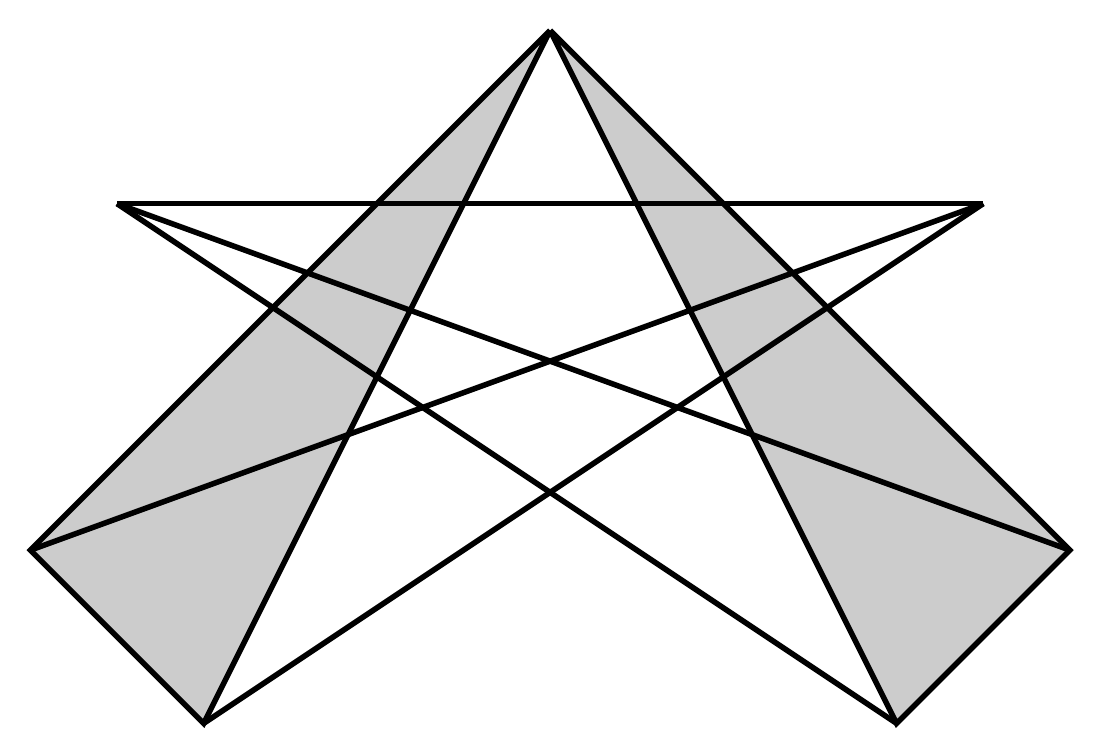
\begin{tikzpicture}[scale=2.2]
        \filldraw[fill=black!20!white, draw=black, line width=2](0, 0)--(-3, -3)--(-2, -4)--(0, 0);
        \filldraw[fill=black!20!white, draw=black, line width=2](0, 0)--(3, -3)--(2, -4)--(0, 0);
        \path[line width=2] 
	        (-2.5, -1) edge (2, -4)
            (-2.5, -1) edge (3, -3)
         (2.5, -1) edge (-2, -4)
  	        (2.5, -1) edge[line width=2] (-2.5, -1)
            (2.5, -1) edge (-3, -3);
        

        \end{tikzpicture}
        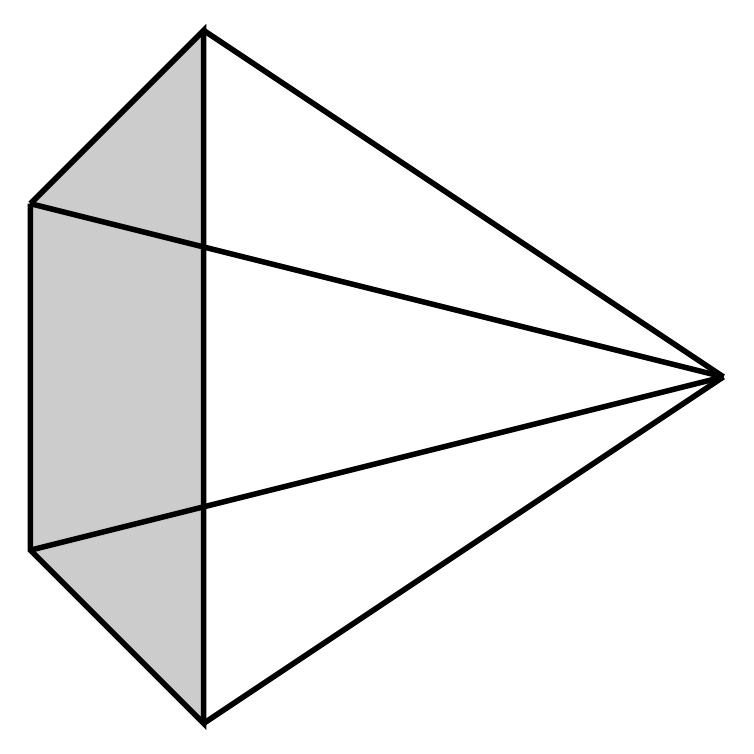
\begin{tikzpicture}[scale=2.2]
        \filldraw[fill=black!20!white, draw=black, line width=2](0, 1)--(0, -1)--(1, -2)--(1, 2)--(0, 1);

        \path[line width=2] 
        	(0, 1) edge (4, 0)
	        (0, -1) edge (4, 0)
            (1, 2) edge (4, 0)
            (1, -2) edge (4, 0);

        \end{tikzpicture}
        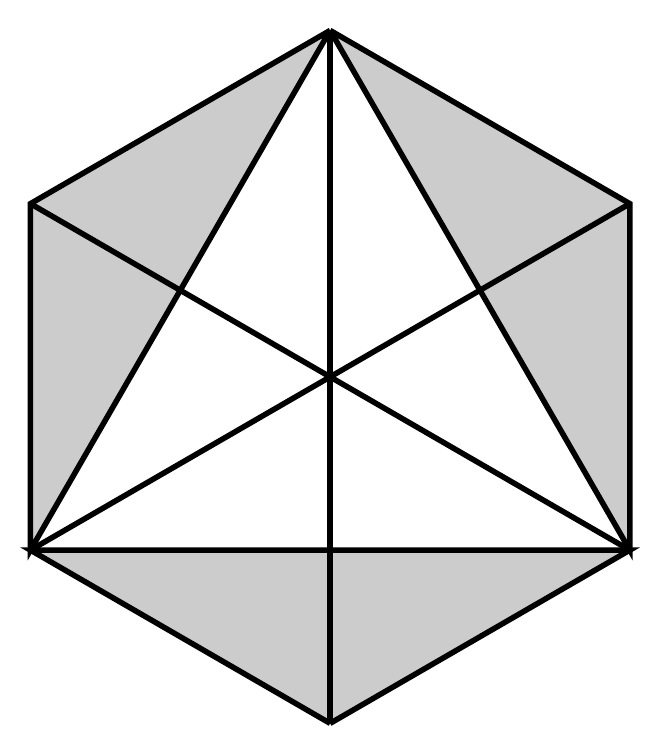
\begin{tikzpicture}[scale=2.2]
        \filldraw[fill=black!20!white, draw=black, line width=2](0, 2)--(1.73, 1)--(1.73, -1)--(0,2);
        \filldraw[fill=black!20!white, draw=black, line width=2](0, 2)--(-1.73, 1)--(-1.73, -1)--(0,2);
        \filldraw[fill=black!20!white, draw=black, line width=2](0, -2)--(1.73, -1)--(-1.73, -1)--(0,-2);
        \path[line width=2] 
	        (0, 2) edge (0, -2)
            (1.73, 1) edge (-1.73, -1)
            (1.73, -1) edge (-1.73, 1);

        \end{tikzpicture}
	\end{tikzfigure}

    }
    
    \vspace{0.3in}
    
    
    }
    

%------------------------------------------
% Second column
%------------------------------------------
    \column{0.4}
    
    
    \block{Planar Results}{
    
    
\theorem{ 
%\label{thm:conv-thrackle}
	Previous conjecture holds in the case that the vertex sets of $C_i, C_j$ are 
	disjoint whenever $C_i, C_j$ are both 2-dimensional.
}


%Each vertex is incident to at most one $2$-dimensional set. Therefore, the neighborhood of a given vertexconsists of some rays along with at most one wedge, which represents a $2$-dimensional convex set. 

\emph{Proof Approach:}
We describe a surjection from a subset of the vertices onto the set of convex sets. Each vertex selects at most one incident set~$C_i$ using the fact that for any vertex sets can only span $(0,\pi)$ interval around the vertex if they are to intersect. We can then break down the cases based on wedge and ray placement and prove by contradiction.

\vspace{0.3in}
    
    \theorem{ 
%\label{thm:comb-thrackle}
	Let $C_1, \dots, C_m$ be sets and suppose there exists a transversal of their pairwise intersections~$W$, 
	that is $|C_i\cap C_j \cap W|=1$ for all $i\ne j$. Then $m \le |W|$.
}

%\begin{proof}
%Create a graph where the vertices represent the sets $C_i$ and there is an edge between the vertices if the two corresponding sets intersect. 
%Since every pair of sets must intersect, this graph will be the complete graph on $m$ vertices,~$K_m$.
%Any point of the transversal set~$W$ induces a complete subgraph of sets it intersects. Therefore $W$ induces 
%a decomposition of the complete graph into complete subgraphs. The complete graph $K_m$ cannot be 
%decomposed into less than $m$ complete subgraphs; see de Brujin and Erd\H{o}s~\cite{erdos1948}. 
%Thus~${m\le |W|}$.
%\end{proof}
\emph{Proof Approach:}
If we create a graph with vertices being the sets and edges are incidence then we will see a tiling of the complete graph by complete subgraphs. The complete graph $K_m$ cannot be decomposed into less than $m$ complete subgraphs; see de Brujin and Erd\H{o}s~\cite{erdos1948}.
    }
    
    
 \block{Examples of Higher Dimensional Thrackles \vspace{-0.47cm}}{ 

\begin{minipage}{8in}
	    An interesting pure thrackle constructed from a traditional tight thrackle. All of the egdes are coned to the blue vertex and the indicated vertices are coned to the red vertex.

 \begin{tikzfigure}%[blahdida]     


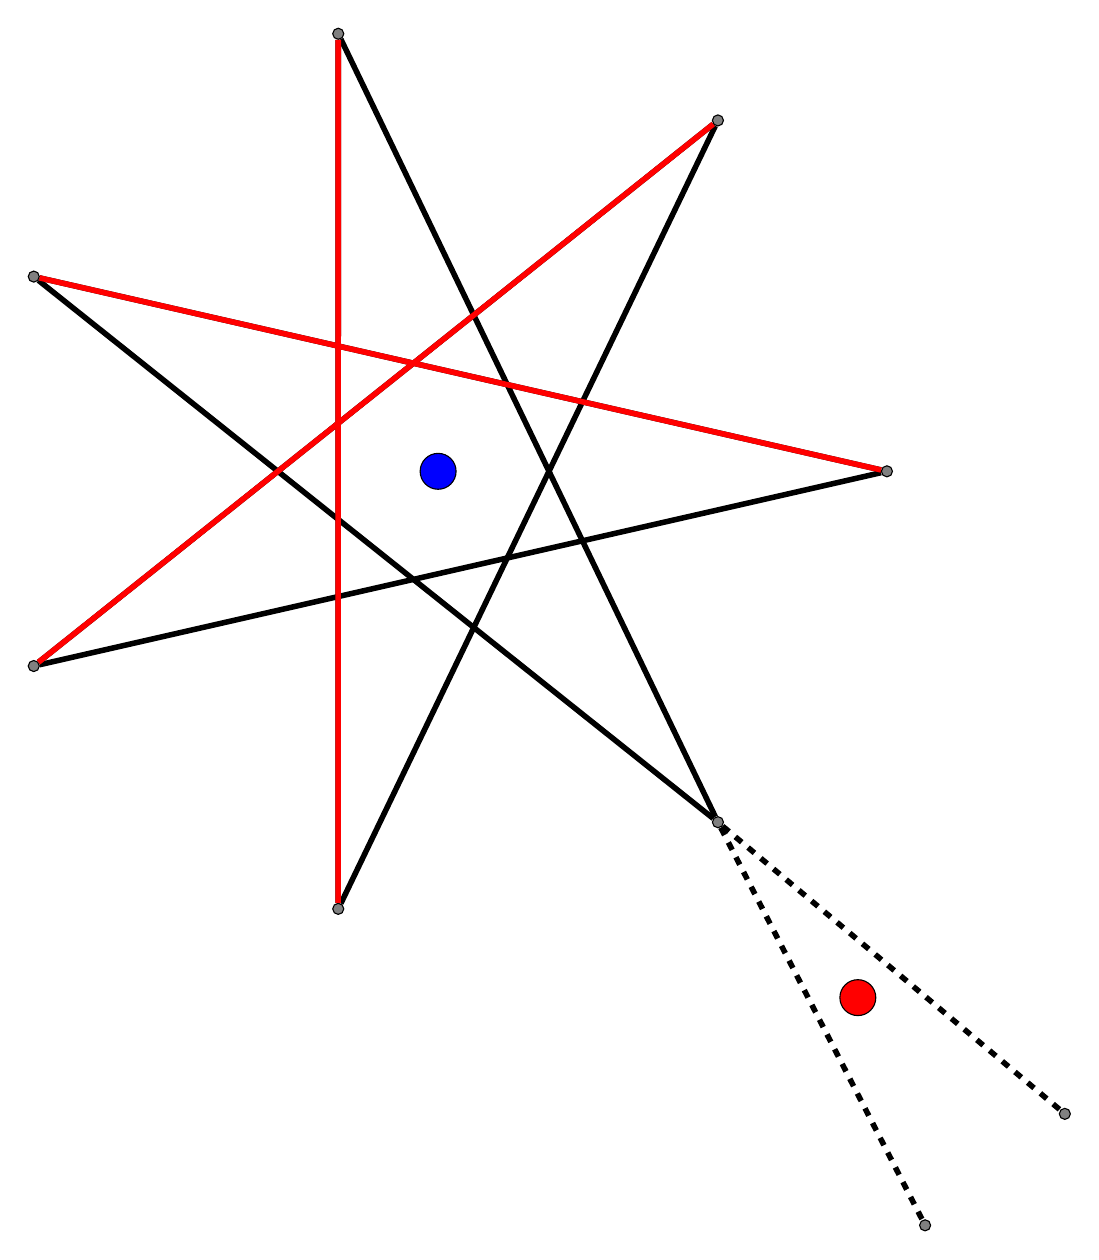
\begin{tikzpicture}[scale=1.9]
 \tikzstyle{every node}=[circle, draw, fill=black!50,
                       inner sep=0pt, minimum width=4pt]
                       
        \filldraw[fill=blue] (0, 0) circle (1.2mm);
 
        \node (A) at (360/7:3){};   %circle(3pt)
        \node (B) at (720/7:3){};
        \node (C) at (1080/7:3){}; %circle(3pt)
        \node (D) at (1440/7:3){}; %circle(3pt)
        \node (E) at (1800/7:3){}; %circle(3pt)
        \node (F) at (2160/7:3){}; %circle(3pt)
        \node (G) at (0:3){};
        %circle(3pt);
        \node (H) at (2200/7:6){};  
        \node (I) at (2120/7:6){};  
        
        \filldraw[fill=red] (2160/7:4.5) circle (1.2mm);
        
        \path[black,-, line width=2]
    (A) edge (D)
    (D) edge (G)
    (G) edge (C)
    (C) edge (F)
    (F) edge (B)
    (B) edge (E)
    (E) edge (A);
    
    \path[dashed,-, line width=2]
    (F) edge (H)
    (F) edge (I);
    
    \path[red,-, line width=2]
    (A) edge (D)
    (G) edge (C)
    (B) edge (E);
    

        
\end{tikzpicture}
\end{tikzfigure}
	\end{minipage}
	\hspace{0.5in}
	\begin{minipage}{8in}
	    This example shows that $m\le |W|$ does not hold for higher dimensions and is an example of a non-pure thrackle.

\vspace{1.25in}

\begin{tikzfigure}%[blahdida]  
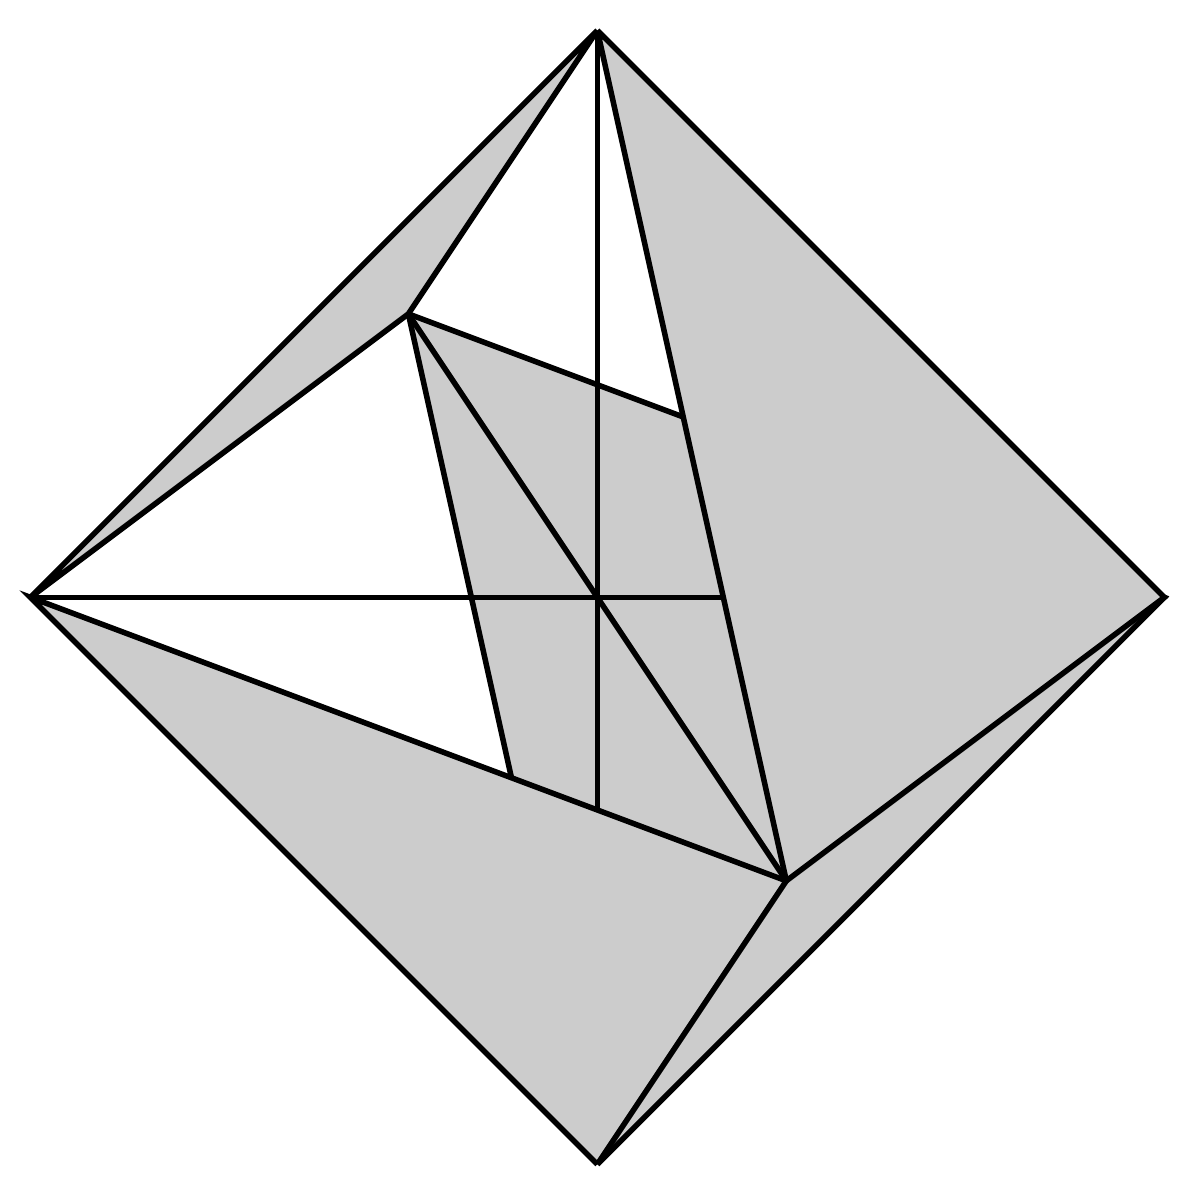
\begin{tikzpicture}[scale=2.4]
 \tikzstyle{every node}=[circle, draw, fill=black!50,
                       inner sep=0pt, minimum width=4pt]
                       
\filldraw[fill=black!20!white, draw=black, line width=2](0, -3)--(-1, 1.5)--(3, 0)--(0,-3);

 \path[black,-, line width=2]
    (-1,1.5) edge (1,-1.5)
    (0,3) edge (0,-3)
    (3,0) edge (-3,0);

\filldraw[fill=black!20!white, draw=black, line width=2](0, -3)--(1, -1.5)--(-3, 0)--(0,-3);

    
 \filldraw[fill=black!20!white, draw=black, line width=2](0, 3)--(3, 0)--(1, -1.5)--(0,3);
\filldraw[fill=black!20!white, draw=black, line width=2](0, 3)--(-1, 1.5)--(-3, 0)--(0,3);

\end{tikzpicture}
\end{tikzfigure}

%\vspace{0.5in}
	\end{minipage}
 




  


	
}



   
    

     \block{\vspace{-0.77cm}References}{
    
    
	\printbibliography[heading=none]%%%TODO fix bib stuff

    }
    

%----------------------------------------------
% Third column
%----------------------------------------------
 
    \column{0.3}
    



 
         \block{Higher Dimensional Thrackles \vspace{-0.47cm}}{ 
   
   \innerblock{Definitions}{
    
A $d$-dimensional simplicial complex is \emph{pure} if every face is contained in a $d$-dimensional face.
A pure simplicial complex $K$ of dimension~$d$ is called \emph{$d$-thrackle} if there is a continuous map
${f \colon K \longrightarrow \R^{d+1}}$ such that
\begin{enumerate}
	\item the restriction of~$f$ to any facet is an embedding,
	\item any two facets intersect in a $(d-1)$-ball,
	\item intersections between faces are \emph{stable}, that is, there is an $\varepsilon > 0$ such that any 
		homotopy that moves points by at most $\varepsilon$ cannot remove the intersection.
\end{enumerate}

The $(d-1)$-faces of a $d$-thrackle are called \emph{ridges}.
If the map $f$ is linear on each facet then we call $K$ \emph{linear $d$-thrackle}.

}

The staright edged traditional thrackle graphs correspond to non-linear $1$-thrackles.

\vspace{0.4in}

\theorem{
%\label{thm:thrackle-highdim}
	A linear $(d-1)$-thrackle with $m$ facets and $n$ ridges satisfies $dm\le 2n$.
}

%\begin{proof}
\emph{Proof Approach:}
Suppose there is a $(d-1)$-thrackle $K$ with $m$ facets and $n$ ridges such that $dm > 2n$ and a
a minimal counterexample. Fix an $f$ that will embed $K$

\begin{itemize}
\item There is a ridge $\tau$ contained in at least three facets $\sigma_1,\sigma_2,\sigma_3$

\item We can examine the hyperplanes that are spanned by $f(\sigma_i)$

\item We can see that some hyperplane $H$ will have an image of one of the facets on the other side of it

\item This means we could remove the facet corresponding to $H$ and get a smaller counterexample
\end{itemize}

%The simplicial complex $K$ contains a ridge $\tau$ that is contained in at least three facets. Let $\sigma_1,
%\sigma_2, \sigma_3$ be three facets incident to~$\tau$. Fix any affine map ${f \colon K \longrightarrow \R^d}$
%that realizes $K$ as a linear $(d-1)$-thrackle. Since $f$ embeds each facet, the $(d-1)$-simplices $f(\sigma_i)$
%span affine hyperplanes~$H_i$. These hyperplanes intersect in the $(d-2)$-plane spanned by~$f(\tau)$,
%and at most two of the hyperplanes can coincide. Thus at least one of the hyperplanes $H_j$ leaves the~$f(\sigma_i)$,
%$i \ne j$, on different sides of it, meaning that $f(\sigma_i) \setminus f(\tau)$, $i \ne j$, are contained in different 
%open halfspaces determined by~$H_j$. We claim that $\sigma_j$ is only adjacent to other facets through~$\tau$
%and not through any other ridge. This is because any facet~$\sigma$ that shares a ridge with~$\sigma_j$
%has its image $f(\sigma)$ entirely contained in one closed halfspace determined by~$H_j$. But unless $\sigma$
%contains $\tau$ the $(d-1)$-simplex $f(\sigma)$ cannot intersect both $f(\sigma_i)$, $i \ne j$, in $(d-2)$-balls.

%Removing $\sigma_j$ yields a $(d-1)$-thrackle with $m-1$ facets and $n-d+1$ ridges. Now $d(m-1) =dm-d > 2n-d
%\ge 2(n-d+1)$ and thus we obtained a counterexample with fewer facets than~$K$, in contradiction to the 
%minimality of~$K$.
%\end{proof}
	
    }
    
    
    
    
   
       \block{Future Work \& Acknowlegements}{
    Higher dimensional thrackles are under more restrictions so might be an easier context under which to look at the traditional thrackle conjecture. A higher dimensional thrackle conjecture could imply the traditional thrackle conjecture.
    
       \begin{tikzfigure}
	    \begin{tikzpicture}
		\begin{scope}[scale=0.85, transform shape]
		    \draw (-4.5in,0) node {\includegraphics[height=1.2in]{./cornelllogo.png}} ;
		    \draw (-2.5in,0) node {\includegraphics[height=1.1in]{./NEU-logo.png}} ;
		    \draw (1in,-0.25) node {\includegraphics[height=1.3in]{./Princeton_University_Logo_09.png}} ;
		    \draw (-0.7in,-0.25) node {\includegraphics[height=1.3in]{./wblogo.png}} ;
		    %\draw (3.5in,0in) node %{\includegraphics[height=1.4in]{./macalester_logo.png}} ;
		    %\draw (6in,0) node {\includegraphics[height=1.4in]{./cu_logo.eps}} ;
		\end{scope}
	    \end{tikzpicture}
	\end{tikzfigure}

    
    
    
     \large This research was performed during the 2016 Cornell University Summer Program for Undergraduate Research.  In addition this research was supported by Princeton University Mathematics Department, Northeastern University Mathematics Department, the Northeastern University Scholars Program and a Watson--Brown Foundation scholarship. 


    }

   

   %\block{Acknowledgements}{


    
%}
    
   




	%----------------------------------------------
	% Logo block
	%----------------------------------------------
	

\end{columns}
%\node [above right,
%       outer sep=0pt,
%       minimum width=\paperwidth-2*\pgflinewidth,
%       minimum height=1cm,
%       align=center,font=\Huge,
%       draw,fill=red] at ([shift={(0.5*\pgflinewidth,0.5*\pgflinewidth)}]bottomleft) {$^1$Tufts University, $^2$University of Nebraska-Lincoln, $^3$Boise State University, $^4$Macalester College, $^5$Cornell University};
       
       
\end{document}
